\documentclass[twoside,10pt]{article}

% this stuff just has to be in here so it doesn't choke
% on the stuff that I put in for typesetting the submission version.
\newcommand{\AuthorAddresses}{}
\newcommand{\KeyWords}{}
\newcommand{\CorrespondingAuthor}{}
\newcommand{\RunningTitle}{}


%!TEX root = main.tex


%%%%% THIS IS THE SECTION WHERE THE AUTHOR PUTS IN ALL OF THEIR TITLE AND AFFILIATION
%%%%% INFORMATION AND  A FEW OTHER THINGS
\newcommand{\myTitle}{A multipurpose microhaplotype panel for genetic analysis of California Chinook salmon}
\title{\myTitle}

% redefine this to make author list. Note affiliation symbols are done manually.
% All caps tends to look better
\newcommand{\myAuthors}{Eric C. Anderson$^{1,\S}$, Anthony J. Clemento$^{1,2}$, Matthew A. Campbell$^{1,2\dagger}$, Devon E. Pearse$^{1,2}$, Anne K. Beulke$^{1,3}$, Cassie Columbus$^{1,2}$, Ellen Campbell$^{1,2}$, Neil F. Thompson$^{1,2\ddag}$, John Carlos Garza$^{1,2,\S}$}
\author{Eric C. Anderson$^{1,2}$, Anthony J. Clemento$^{1,2}$, Matthew A. Campbell$^{1,2,\dagger}$, Devon E. Pearse$^{1,2}$, Anne K. Beulke$^{1,3}$, Cassie Columbus$^{1,2}$, Ellen Campbell$^{1,2}$, Neil F. Thompson$^{1,2,\ddag}$, John Carlos Garza$^{1,2,\S}$}


% redefine to make the affiliation list.  Note symbols are done manually
\newcommand{\myAffiliations}{
$^1$Southwest Fisheries Science Center, National Marine Fisheries Service, NOAA, Santa Cruz, California, USA. $^2$Institute for Marine Sciences, University of California, Santa Cruz, USA. $^3$Department of Ocean Sciences, University of California, California, Santa Cruz, USA. $^\dagger$Current address: Centre for Carbon, Water and Food, The University of Sydney, 380 Werombi Road, NSW 2570, Australia. $^\ddag$Current address: Pacific Shellfish Research Unit, Agricultural Research Service, US Department of Agriculture, Newport, Oregon, USA.
}

\renewcommand{\AuthorAddresses}{\myAffiliations}

\renewcommand{\KeyWords}{Genetic stock identfication, population assignment, parentage based tagging, amplicon sequencing}

\renewcommand{\CorrespondingAuthor}{eric.anderson@noaa.gov,~carlos.garza@noaa.gov}


% the email address for the corresponding author
\newcommand{\myEmailAddress}{eric.anderson@noaa.gov,~carlos.garza@noaa.gov}
\newcommand{\myEmailFootnote}{$^\S$}

% here you can put your very own copyright notice
\newcommand{\myCopyright}{\copyright US Federal Government work in the public domain in the USA}

% here you can put a running title (a short title that goes on the left of the
% even pages)
\newcommand{\myRunningTitle}{Microhaplotypes for California Chinook salmon}
\renewcommand{\RunningTitle}{\myRunningTitle}

% and here you put the running author (short listing of authors for the
% upper right header on the odd pages)
\newcommand{\myRunningAuthor}{Anderson et al.}

%%%% DONE WITH AUTHOR/TITLE/ETC INFORMATION DEFINITION
  % Put all the author title stuff in there

% ------
% Fonts and typesetting settings
\usepackage[sc]{mathpazo}
\usepackage[T1]{fontenc}
\linespread{1.05} % Palatino needs more space between lines

\usepackage{microtype}
% ------
% Page layout
\usepackage[labelfont=bf,labelformat=simple,labelsep=quad]{caption}

\usepackage{amsmath}
\usepackage{graphicx}
\usepackage{amssymb}
\usepackage{epstopdf}
\usepackage{amsfonts}
\usepackage{natbib}
\usepackage{xspace}
\usepackage{mathrsfs}
\usepackage{fancyhdr}
\usepackage{cuted}
\usepackage{flushend}
\usepackage{enumerate}
\usepackage{hyperref}
\usepackage{url}
\usepackage{scalerel}
\usepackage{color}
\usepackage{xr}

\usepackage{draftwatermark}
\SetWatermarkText{DRAFT}
\SetWatermarkScale{1}


\externaldocument{main}





\newcommand{\relat}{R}
\newcommand{\relatset}{\mathscr{R}}
\newcommand{\nA}{\mathcal{A}}
\newcommand{\nL}{\mathcal{L}}
\newcommand{\nG}{\mathcal{G}}
\newcommand{\MAF}{\mathrm{MAF}}

\newcommand{\Pe}{\mathrm{P}_\epsilon}
\newcommand{\PR}{\mathrm{P}_\relat}

\newcommand{\bkappa}{\bm{\kappa}}

\newcommand{\comment}[1]{\textcolor{red}{#1}}

\newcommand{\BY}{\mathbf{Y}}
\newcommand{\BX}{\mathbf{X}}
\newcommand{\BC}{\mathbf{C}}
\newcommand{\I}{\mathbb{1}}
\newcommand{\bomega}{\bm{\omega}}

\newcommand{\Exp}{\mathbb{E}}
\newcommand{\Var}{\mathrm{Var}}

\newcommand{\heta}{\hat{\theta}}
\newcommand{\bg}{\bm{g}}

\newcommand{\GG}{\mathscr{G}}

\newcommand{\LFball}{\raisebox{-0.12 em}{
\includegraphics[height=1.02em]{images/Late-fall-run-ball-crop.pdf}}}
\newcommand{\Fball}{\raisebox{-0.12 em}{
\includegraphics[height=1.02em]{images/Fall-run-ball-crop.pdf}}}
\newcommand{\Wball}{\raisebox{-0.12 em}{
\includegraphics[height=1.02em]{images/Winter-run-ball-crop.pdf}}}
\newcommand{\Sball}{\raisebox{-0.12 em}{
\includegraphics[height=1.02em]{images/Spring-run-ball-crop.pdf}}}




%% some handy things for making bold math
\def\bm#1{\mathpalette\bmstyle{#1}}
\def\bmstyle#1#2{\mbox{\boldmath$#1#2$}}
\newcommand{\thh}{^\mathrm{th}}


%% Some pretty etc.'s, etc...
\newcommand{\cf}{{\em cf.}\xspace }
\newcommand{\eg}{{\em e.g.},\xspace }
\newcommand{\ie}{{\em i.e.},\xspace }
\newcommand{\etal}{{\em et al.}\ }
\newcommand{\etc}{{\em etc.}\@\xspace}



%% the page dimensions
\textwidth = 6.5 in
\textheight = 9 in
\oddsidemargin = -0.01 in
\evensidemargin = -0.01 in
\topmargin = -0.7 in
\headheight = 0.25 in
\headsep = 0.25 in
\parskip = 0.0in
\parindent = 0.25in

\setlength{\columnsep}{.4in}


%% change section heading styles
\makeatletter
\setcounter{figure}{0}
\renewcommand{\thefigure}{S\arabic{figure}}
\renewcommand{\thetable}{S\arabic{table}}
\renewcommand{\thesection}{S\arabic{section}}
\renewcommand\section{\@startsection {section}{1}{\z@}%
                                   {-3.5ex \@plus -1ex \@minus -.2ex}%
                                   {1.5ex \@plus 0ex}%
                                   {\normalfont\normalsize\bfseries}}
                                   
%    \renewcommand\subsection{\@startsection{subsection}{2}{\z@}%
%                                     {-3.25ex\@plus -1ex \@minus -.2ex}%
%                                     {1.5ex \@plus .2ex}%
%                                     {\normalfont\small\itshape}}
%
%\renewcommand\subsubsection{\@startsection{subsection}{2}{\z@}%
%                                     {-3.25ex\@plus -1ex \@minus -.2ex}%
%                                     {1.5ex \@plus .2ex}%
%                                     {\normalfont\footnotesize\bfseries}}
\makeatother
%

\fancypagestyle{firststyle}
{
   \fancyhf{}
   \mbox{}   
   \vspace*{1em} 
   \mbox{}\\
        {\LARGE\bf {\sc supplement to:}~~\myTitle \par}
    \mbox{}\\
    \uppercase{\myAuthors}\\
       \mbox{}\\
    {\em \myAffiliations}\\
    \mbox{}\\
    {\small \myEmailFootnote Correspondence: \myEmailAddress}
\mbox{}
\vspace*{4em}\mbox{}


   \lfoot[]{\footnotesize \myCopyright}
}

%% here is what I hope will be fancyplain
\fancyhead{} % clear all header fields
\fancyhead[LE]{{\bf \thepage}~~{\sl \myRunningTitle}}
\fancyfoot[RE,LO]{{\footnotesize \myCopyright}}
\renewcommand{\headrulewidth}{0pt}
\fancyhead[RO]{{\sl \myRunningAuthor}~~{\bf \thepage}}
\cfoot[]{}



\begin{document}


\pagestyle{fancyplain}
\thispagestyle{firststyle}

\tableofcontents
\listoffigures
\listoftables

\clearpage 

{\small
%!TEX root = supplement.tex

\section{Winter-run-associated polymorphism methods and results\label{sec:wrap-methods}}

We used the whole genome sequencing data from \citet{thompson2020complex} to seek variants with
large allele frequency differences between winter-run Chinook salmon and all the other
Chinook salmon ecotypes in the Central Valley of California (CCV).  Because winter-run Chinook are
already highly differentiated from all others, we did not pursue an association study as used
for identifying the late-fall-run associated variants.  Rather, we first identified regions with a high
density of variants with large allele frequency differences between winter-run and non-winter-run
fish in the CCV\@. Subsequently we identified SNPs within those regions with particularly
large allele frequency differences.  This approach was taken to avoid targeting single, isolated SNPs
with large allele frequency differences that may have resulted merely from sampling variation, which was a
concern because we had whole genome sequencing data from only 16 winter run fish.

More specifically, we calculated allele frequencies for 16 winter-run fish and 84 non-winter-run
fish from the  \citet{thompson2020complex} variant data VCF files using ANGSD version~0.921.
Sites were retained if at least 62.5\% of samples in each group had read data (10 of 16 for the
winter run and 50 of 80 for the non-winter run), resulting in 7,295,001 SNPs for downstream
analysis.  We first investigated the distribution throughout the genome of $|d|$, the absolute difference
of the alternate allele frequency between the two groups  (Fig.~\ref{fig:wrap-absdiff}). This revealed
that many loci had large values of $|d|$, but there were several
regions in the genome, in particular, with prominent peaks in allele frequency difference and one
or more SNPs apparently fixed for alternate alleles between the two sample groups.  

To leverage information from multiple SNPs to identify regions in the genome with large
allele frequency differences, we calculated the fraction of SNPs with $|d| > 0.5$ that also
had $|d| > 0.9$ within non-overlapping 100 kb sliding windows throughout the genome. This metric indicated
several prominent peaks.  We focused on all of those
100 kb windows in which more than 12.4\% of sites with $|d|>0.5$ also had $|d|>0.9$ which were
also adjacent to at least one window in which $>10\%$ of sites with $|d|>0.5$ also had $|d|>0.9$ 
(Fig.~\ref{fig:wrap-slide-window}).  Within the windows found on four different chromosomes using
the above criteria, we then attempted to design amplicons to type the SNPs at a subset of the sites
within each window.  We chose all sites with $|d|>0.975$, as well as the 8 SNPs on each chromosome
with the highest values of $|d|$, yielding 61 candidate SNPs (Fig.~\ref{fig:wrap-candi}).  

Some of those 61 candidate SNPs were close enough that it was possible to consider amplifying them
with PCR on 58 different short sequences.  We used Primer3 \citep{untergasser2012primer3} to return
three possible primer-pair designs for each of the 58 sequences and then chose the primer pair
with the fewest penalties, optimal target size, and most consistent
melting temperatures.  One primer pair was dropped from consideration because it
amplified a large indel that was apparent in the sequence data which would have rendered
the sequence too large to efficiently amplify and several others were dropped because the primers
overlapped other amplicons.  Finally, several amplicons with the lowest $|d|$ on chromosome 16
(RefSeq NC\_037112.1) were removed from consideration, leaving us with 48 amplicons to test
for amplification and for evaluation of allele frequencies.

%% Note to self.  The next section is documented in the project at:
%% /Users/eriq/Documents/work/assist/anthony_clemento/WRAP-crunching
These 48 amplicons were amplified and sequenced in 192 fish---96 Feather River spring run
and 96 winter run---on a MiSeq sequencer, and the variants were called using
GATK.  The resulting VCF file was used to estimate allele frequency differences between
winter run and feather river spring.  We also processed the sequence data using
microhaplot (\url{https://github.com/ngthomas/microhaplot}) and visually inspected
loci for consisten allele depth ratio and numbers of haplotypes.  We then chose 24 amplicons for further
testing on the basis of allele frequency differences between Feather River spring run and
winter run, number of haplotypes, and ease of scoring.  These 24 markers were typed on
a variety of fish over the course of a year, and we finally chose three to include in
our California Chinook reference baseline: one amplicon on each of chromosomes
8, 12, and 16.  The estimated frequencies of all the alleles present in the reference baseline
in those three amplicons shows that there are not fixed differences between
winter run and all other reporting units (Table~\ref{tab:wrap-freqs}).



}
\clearpage

{\small
%!TEX root = supplement.tex

%%%%%%%%%%%%%%%%%%%
\begin{figure}
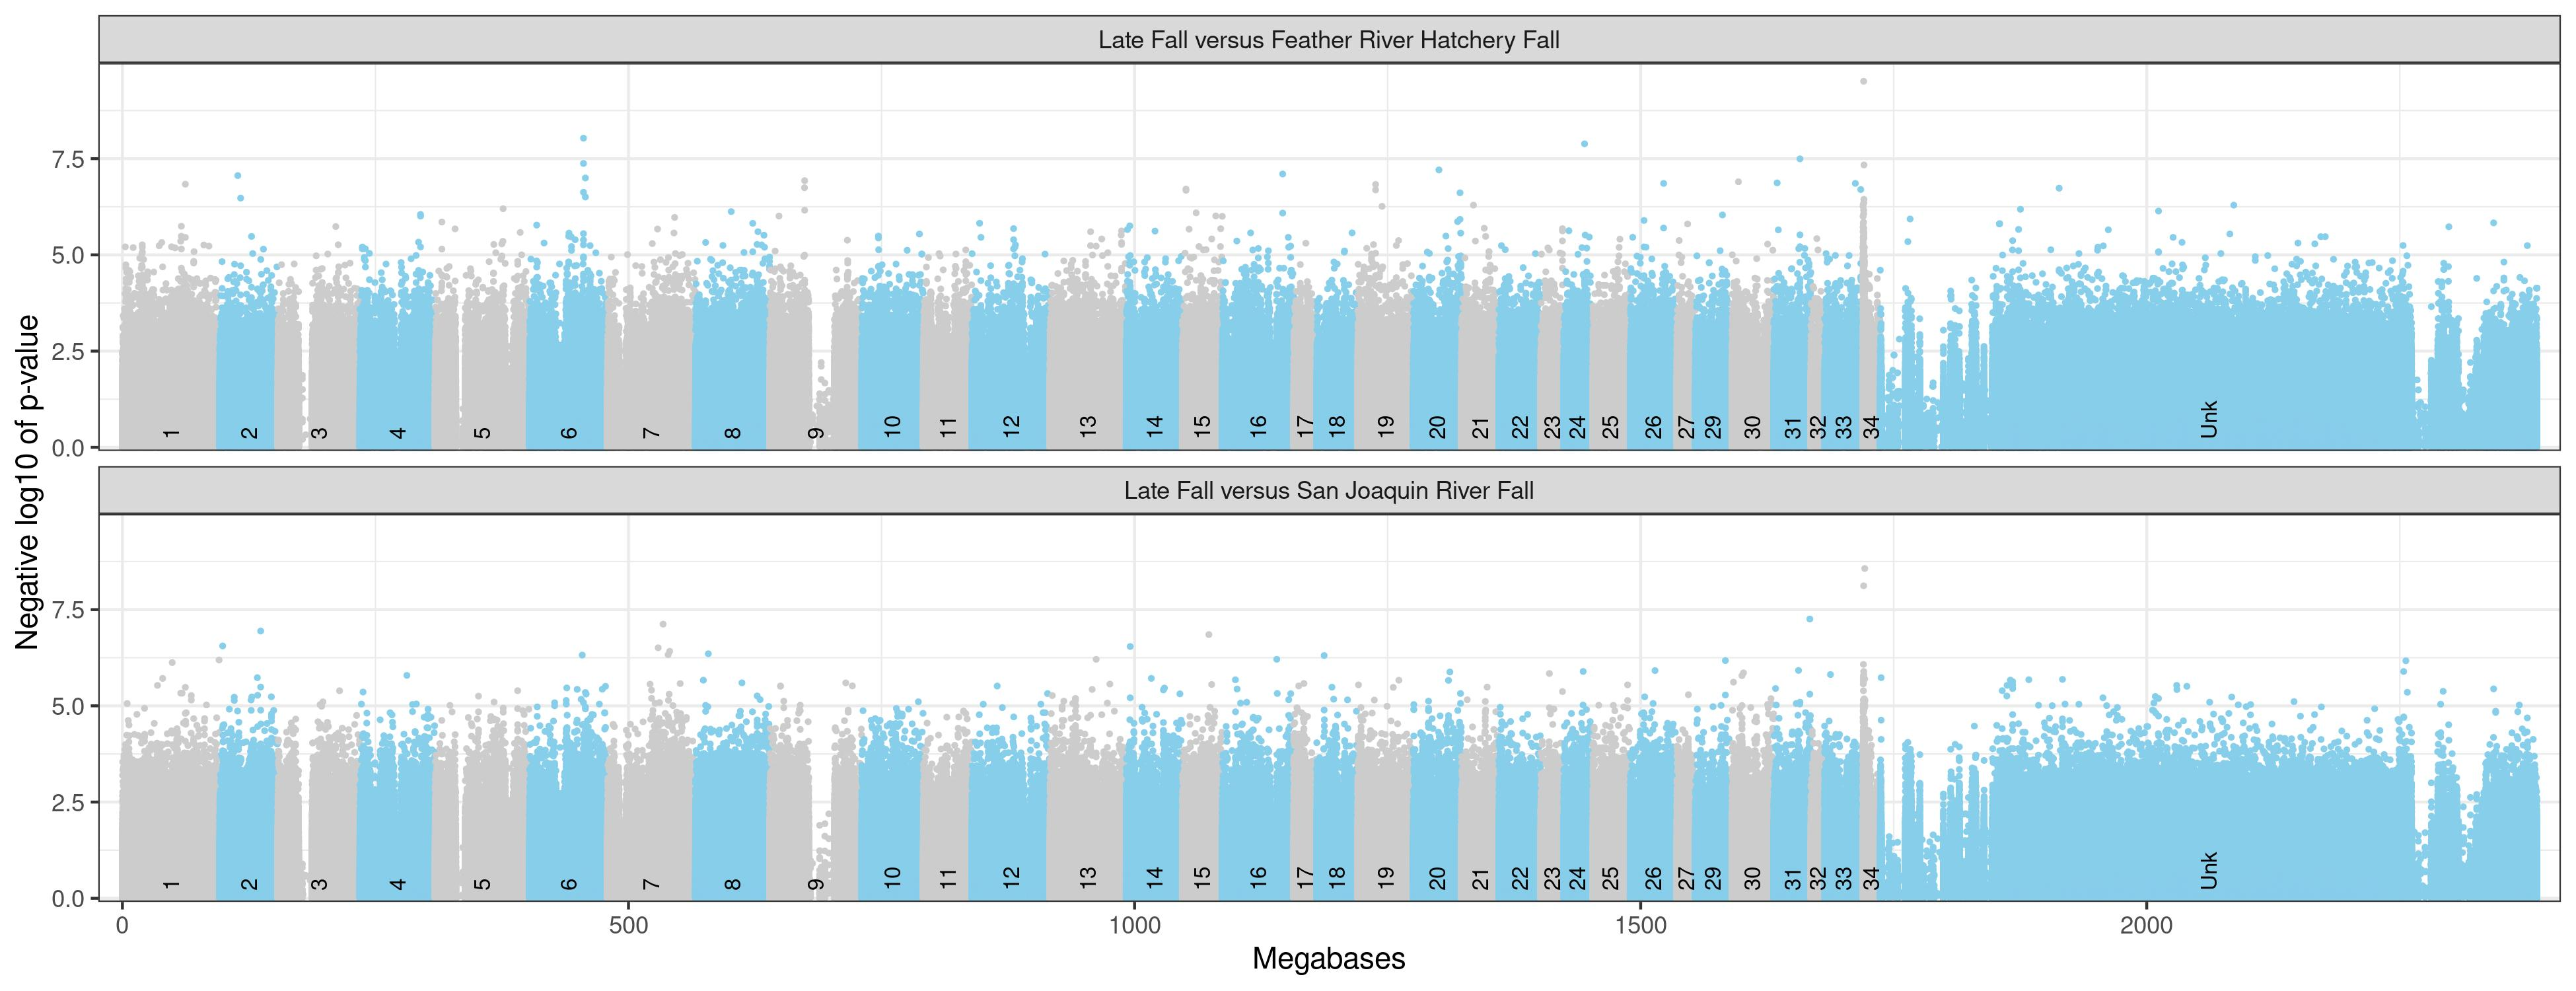
\includegraphics[width=\textwidth]{images/lfar-assoc-faceted.jpg}
\caption[
	Negative log base 10 of association $p$-values for
	individual SNPs for late-fall versus fall run
]{
	\footnotesize Negative log base 10 of association $p$-values for
	individual SNPs for late-fall versus fall run.  $x$ axis shows position in genome (in megabases),
	with color alternating by chromosome, as indicated by numbers above the $x$-axis. ``Unk'' refers
	to unplaced scaffolds in the Otsh\_v1.0 genome assembly \citep{christensen2018chinook}. The 
	upper panel is the comparison between late-fall and Feather River Hatchery fall, while the lower 
	panel is the comparison of late-fall to San Joaquin River fall. 
}
\label{fig:lfar-assoc}
\end{figure}



%%%%%%%%%%%%%%%%%%%%%% 
\begin{figure}
\begin{center}
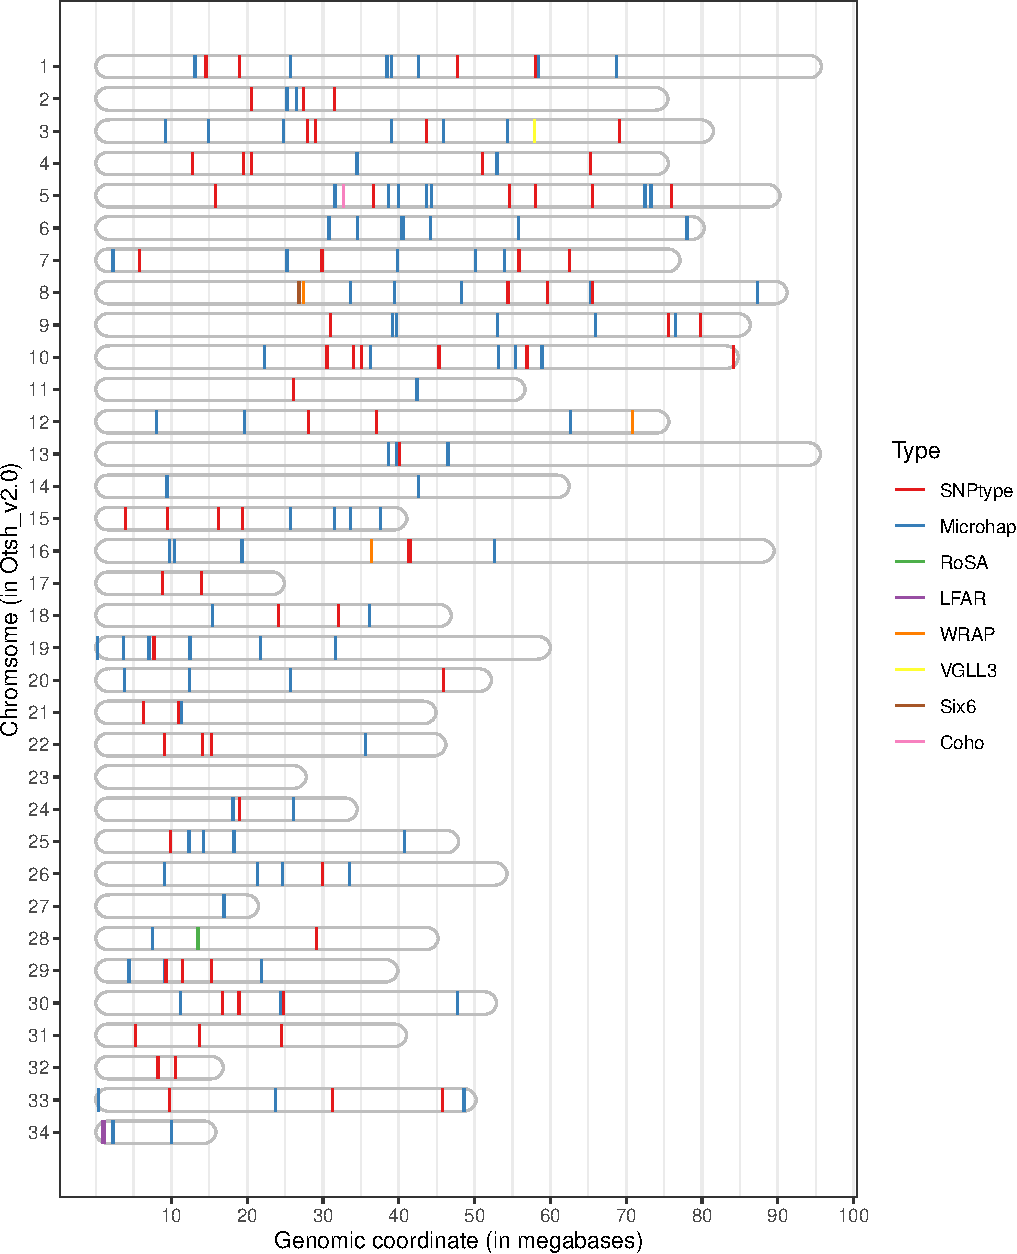
\includegraphics[width=0.7\textwidth]{images/genomic-locations-plot.pdf}
\end{center}
\caption[Genomic locations of amplicons]{\footnotesize Genomic locations of amplicons in the
Otsh\_v2.0 assembly of the Chinook salmon genome.  Color shows type of marker (see main text).
The sex-ID marker is not included here because it aligns to a scaffold that is not part of a
named chromosome/linkage group in the assembly.}
\label{fig:num-alle}
\end{figure}
%%%%%%%%%%%%%%%%%%%%





%%%%%%%%%%%%%%%%%%%%%% 
\begin{figure}
\begin{center}
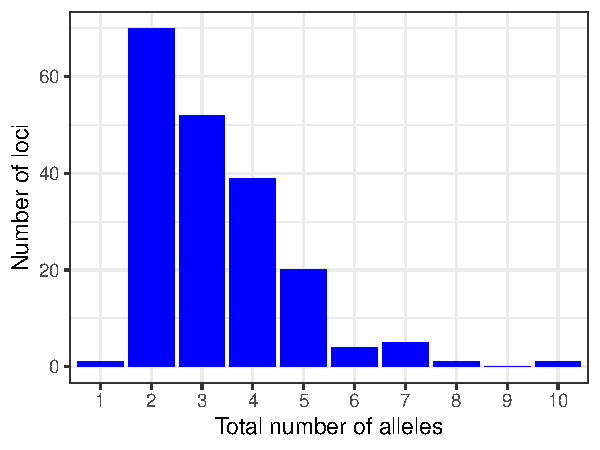
\includegraphics[width=0.7\textwidth]{images/num-alle-barplot.pdf}
\end{center}
\caption[Number of loci with different
total numbers of alleles]{\footnotesize Number of loci with different
total numbers of alleles in the data set. The one amplicon with only
one allele is {\tt Ots\_coho001\_05\_32691399}, which is fixed for alternate alleles
in Chinook vs.\ coho salmon. It is helpful in identifying coho samples that are
misidentified during sampling as Chinook salmon.}
\label{fig:num-alle}
\end{figure}
%%%%%%%%%%%%%%%%%%%%




%%%%%%%%%%%%%%%%%%%%%% 
\begin{figure}
\begin{center}
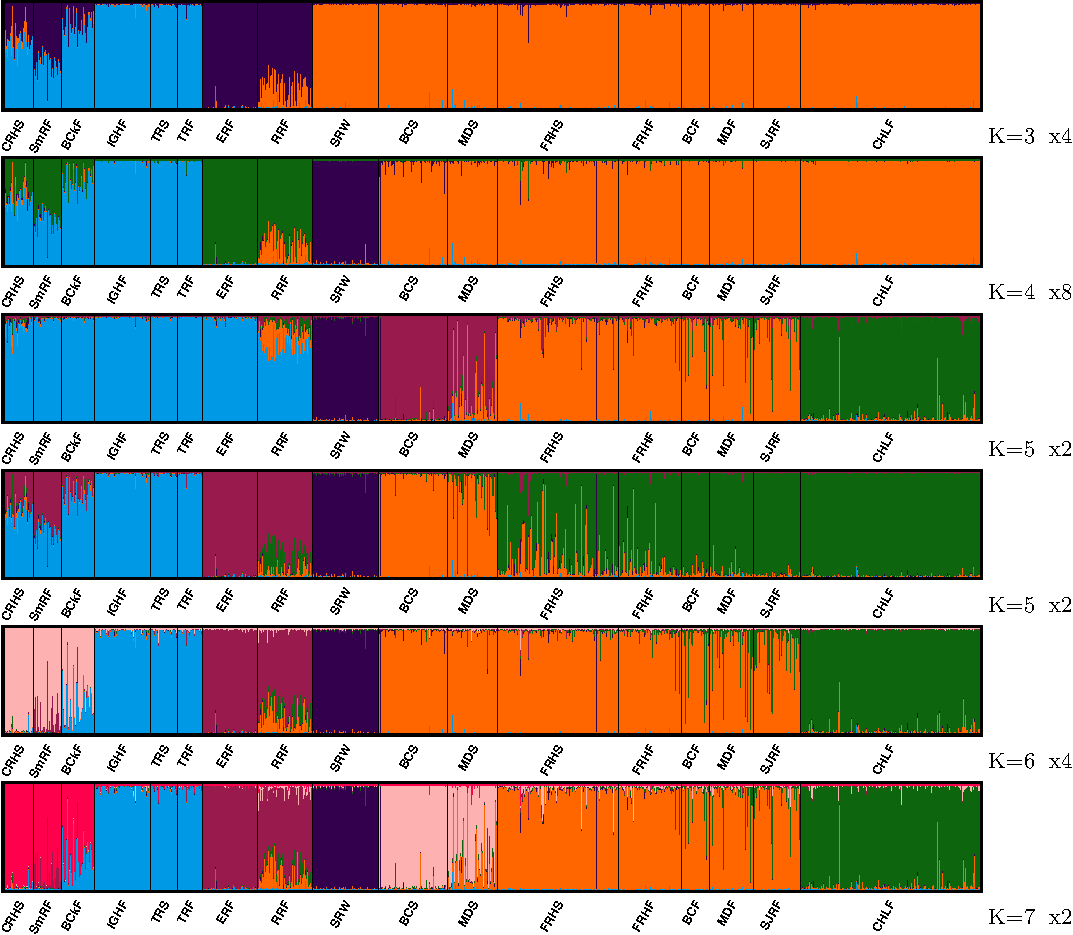
\includegraphics[width=0.7\textwidth]{images/minor-modes-crop.pdf}
\end{center}
\caption[STRUCTURE minor modes found by CLUMPAK]{\footnotesize At each value of $K$
for which a minor mode was found, these plots show them}
\label{fig:minor-modes}
\end{figure}
%%%%%%%%%%%%%%%%%%%%


%%%%%%%%%%%%%%%%%%%%%% 
\begin{figure}
\begin{center}
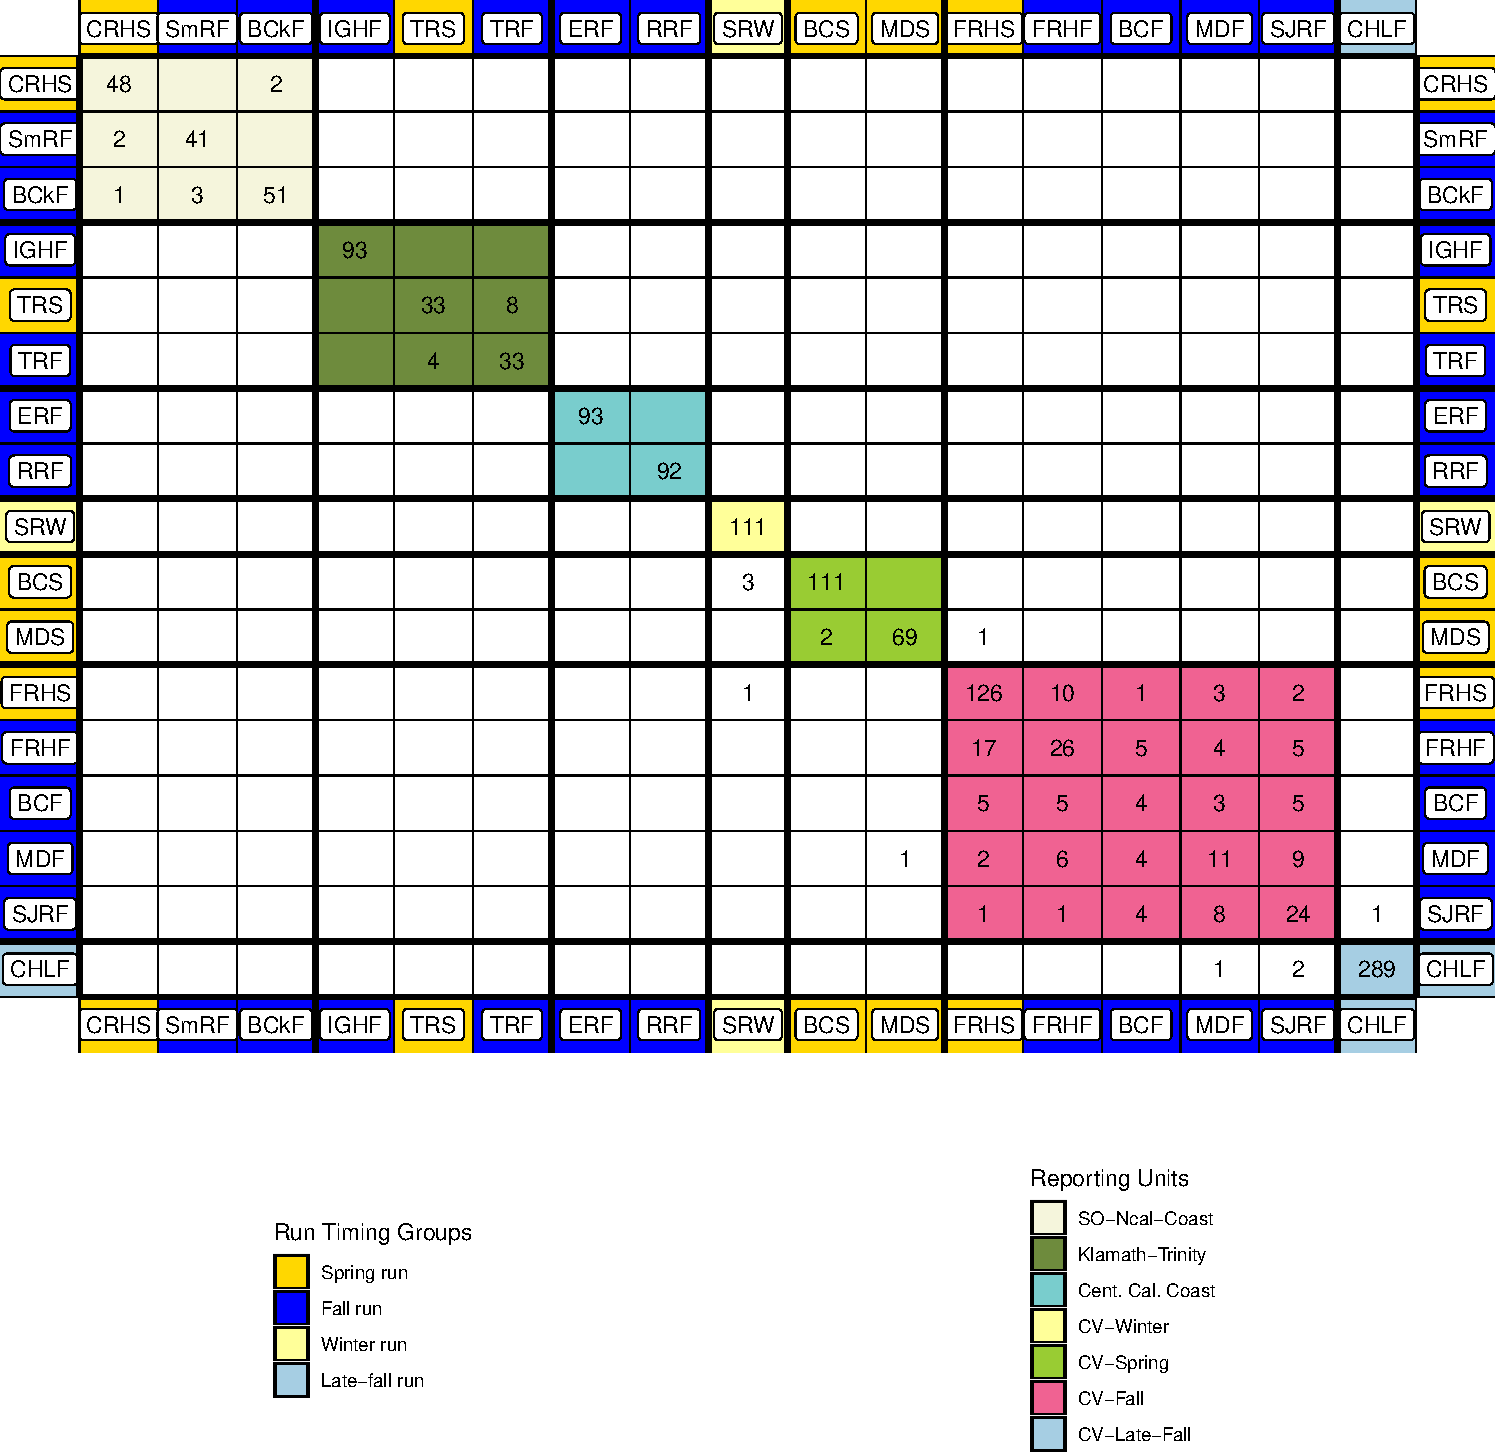
\includegraphics[width=0.8\textwidth]{images/ass-table-80-crop.pdf}
\end{center}
\caption[Assignment table for fish with scaled likelihood $ > 0.8$]{\footnotesize Assignment table
like that in Fig.~\ref{fig:gsi}b in the paper, but constrained so that only fish assigning
to a reporting unit with scaled likelihood greater than 0.8 are included.}
\label{fig:eighty}
\end{figure}
%%%%%%%%%%%%%%%%%%%%





%%%%%%%%%%%%%%%%%%%%%% 
\begin{figure}
\begin{center}
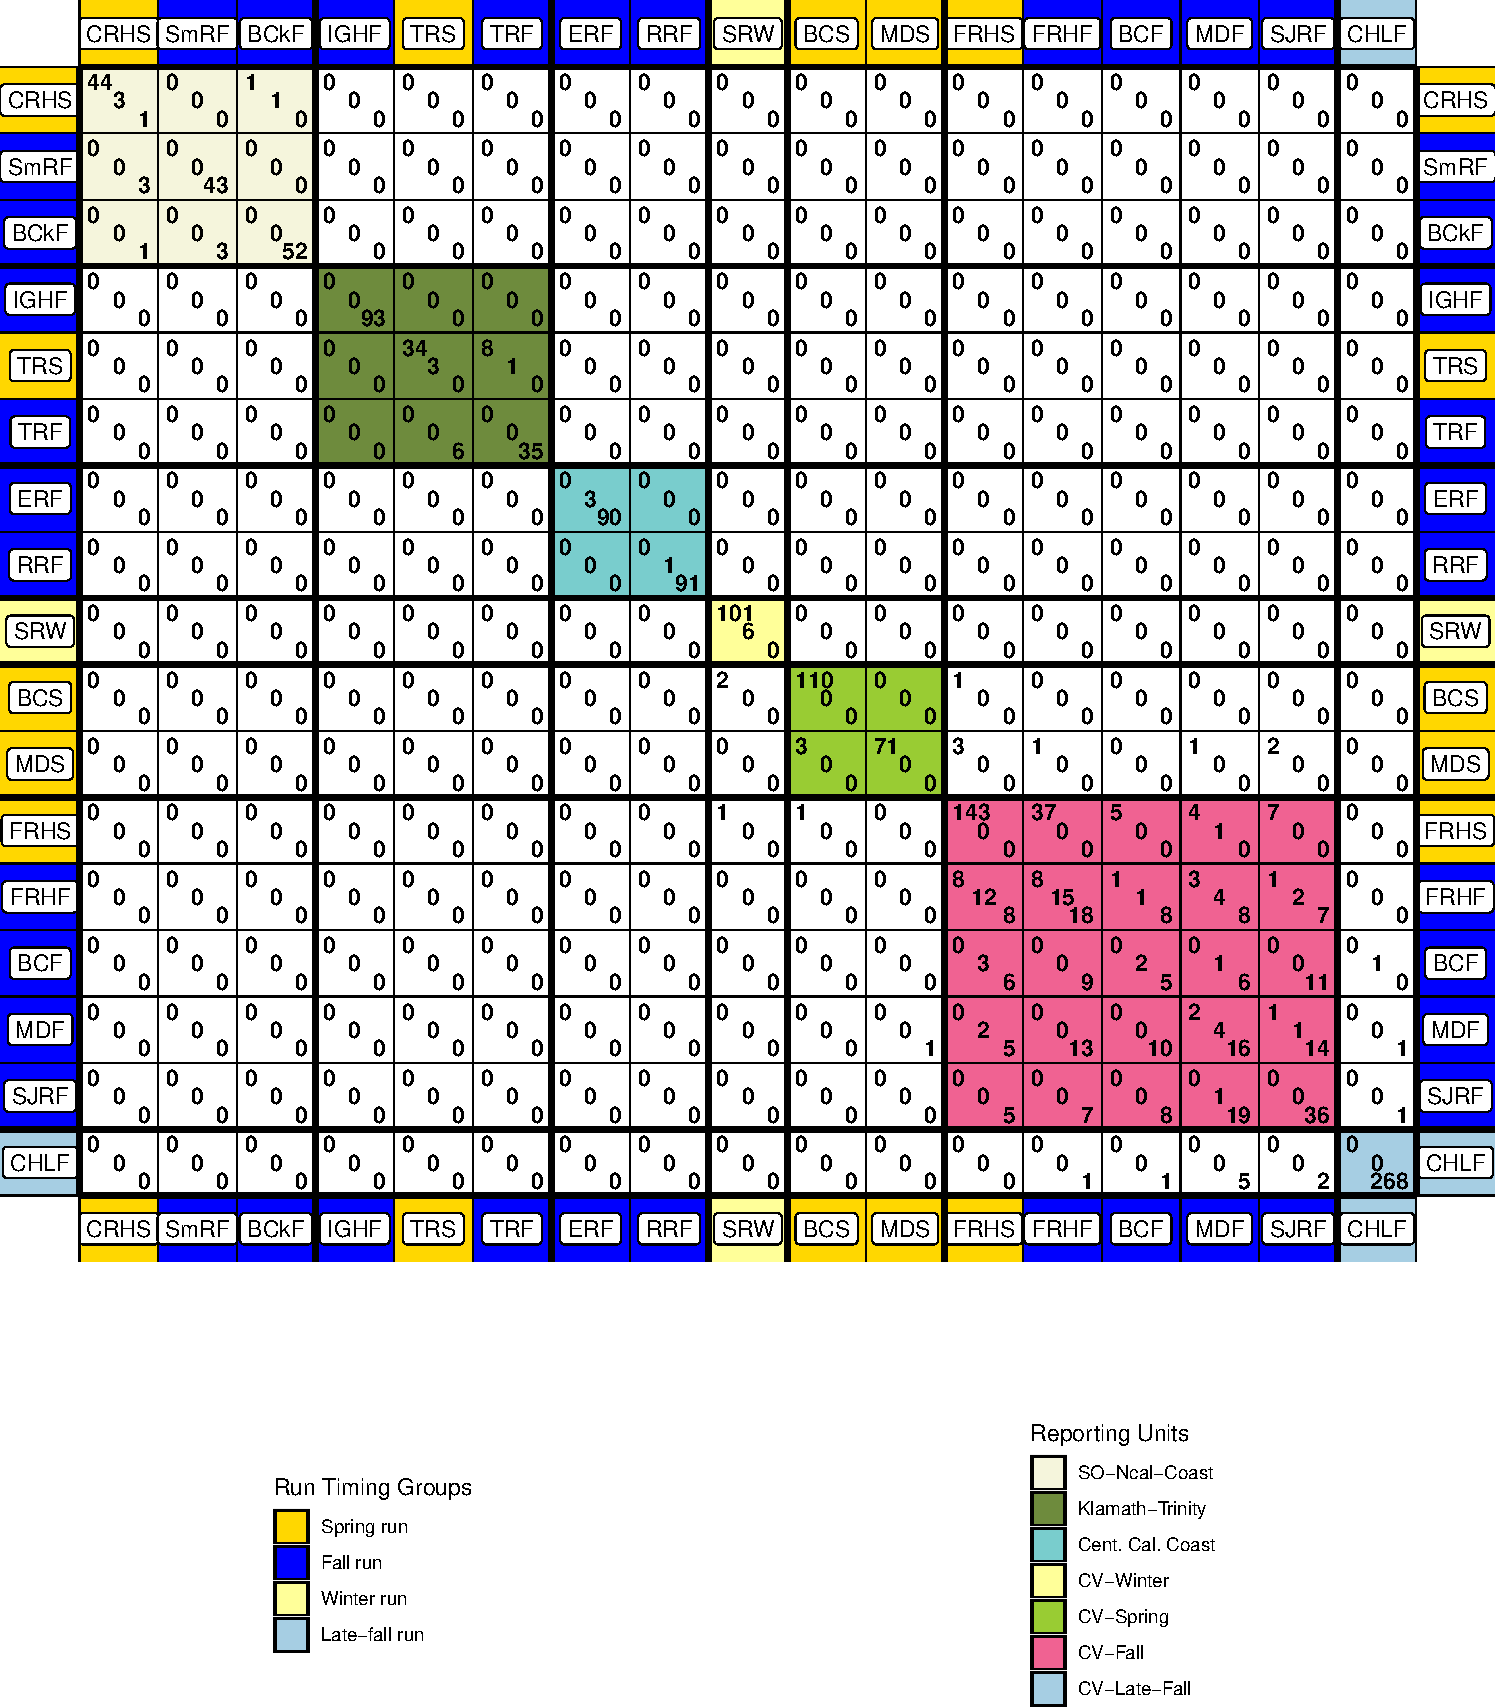
\includegraphics[width=0.8\textwidth]{images/rosa-gsi-table-crop.pdf}
\end{center}
\caption[Assignment table by RoSA genotype]{\footnotesize Assignment table
like that in Fig.~\ref{fig:gsi}b in the paper, but with numbers according to genotypes
at the RoSA. In each cell, the top left entry gives the number of EE (early run allele homozygotes)
genotypes, the middle entry is the number of EL genotypes (heterozygotes), and the bottom
right entry gives the number of LL (late-run homozygote) genotypes. }
\label{fig:rosa-gsi}
\end{figure}
%%%%%%%%%%%%%%%%%%%%



%%%%%%%%%%%%%%%%%%%%%% 
\begin{figure}
\begin{center}
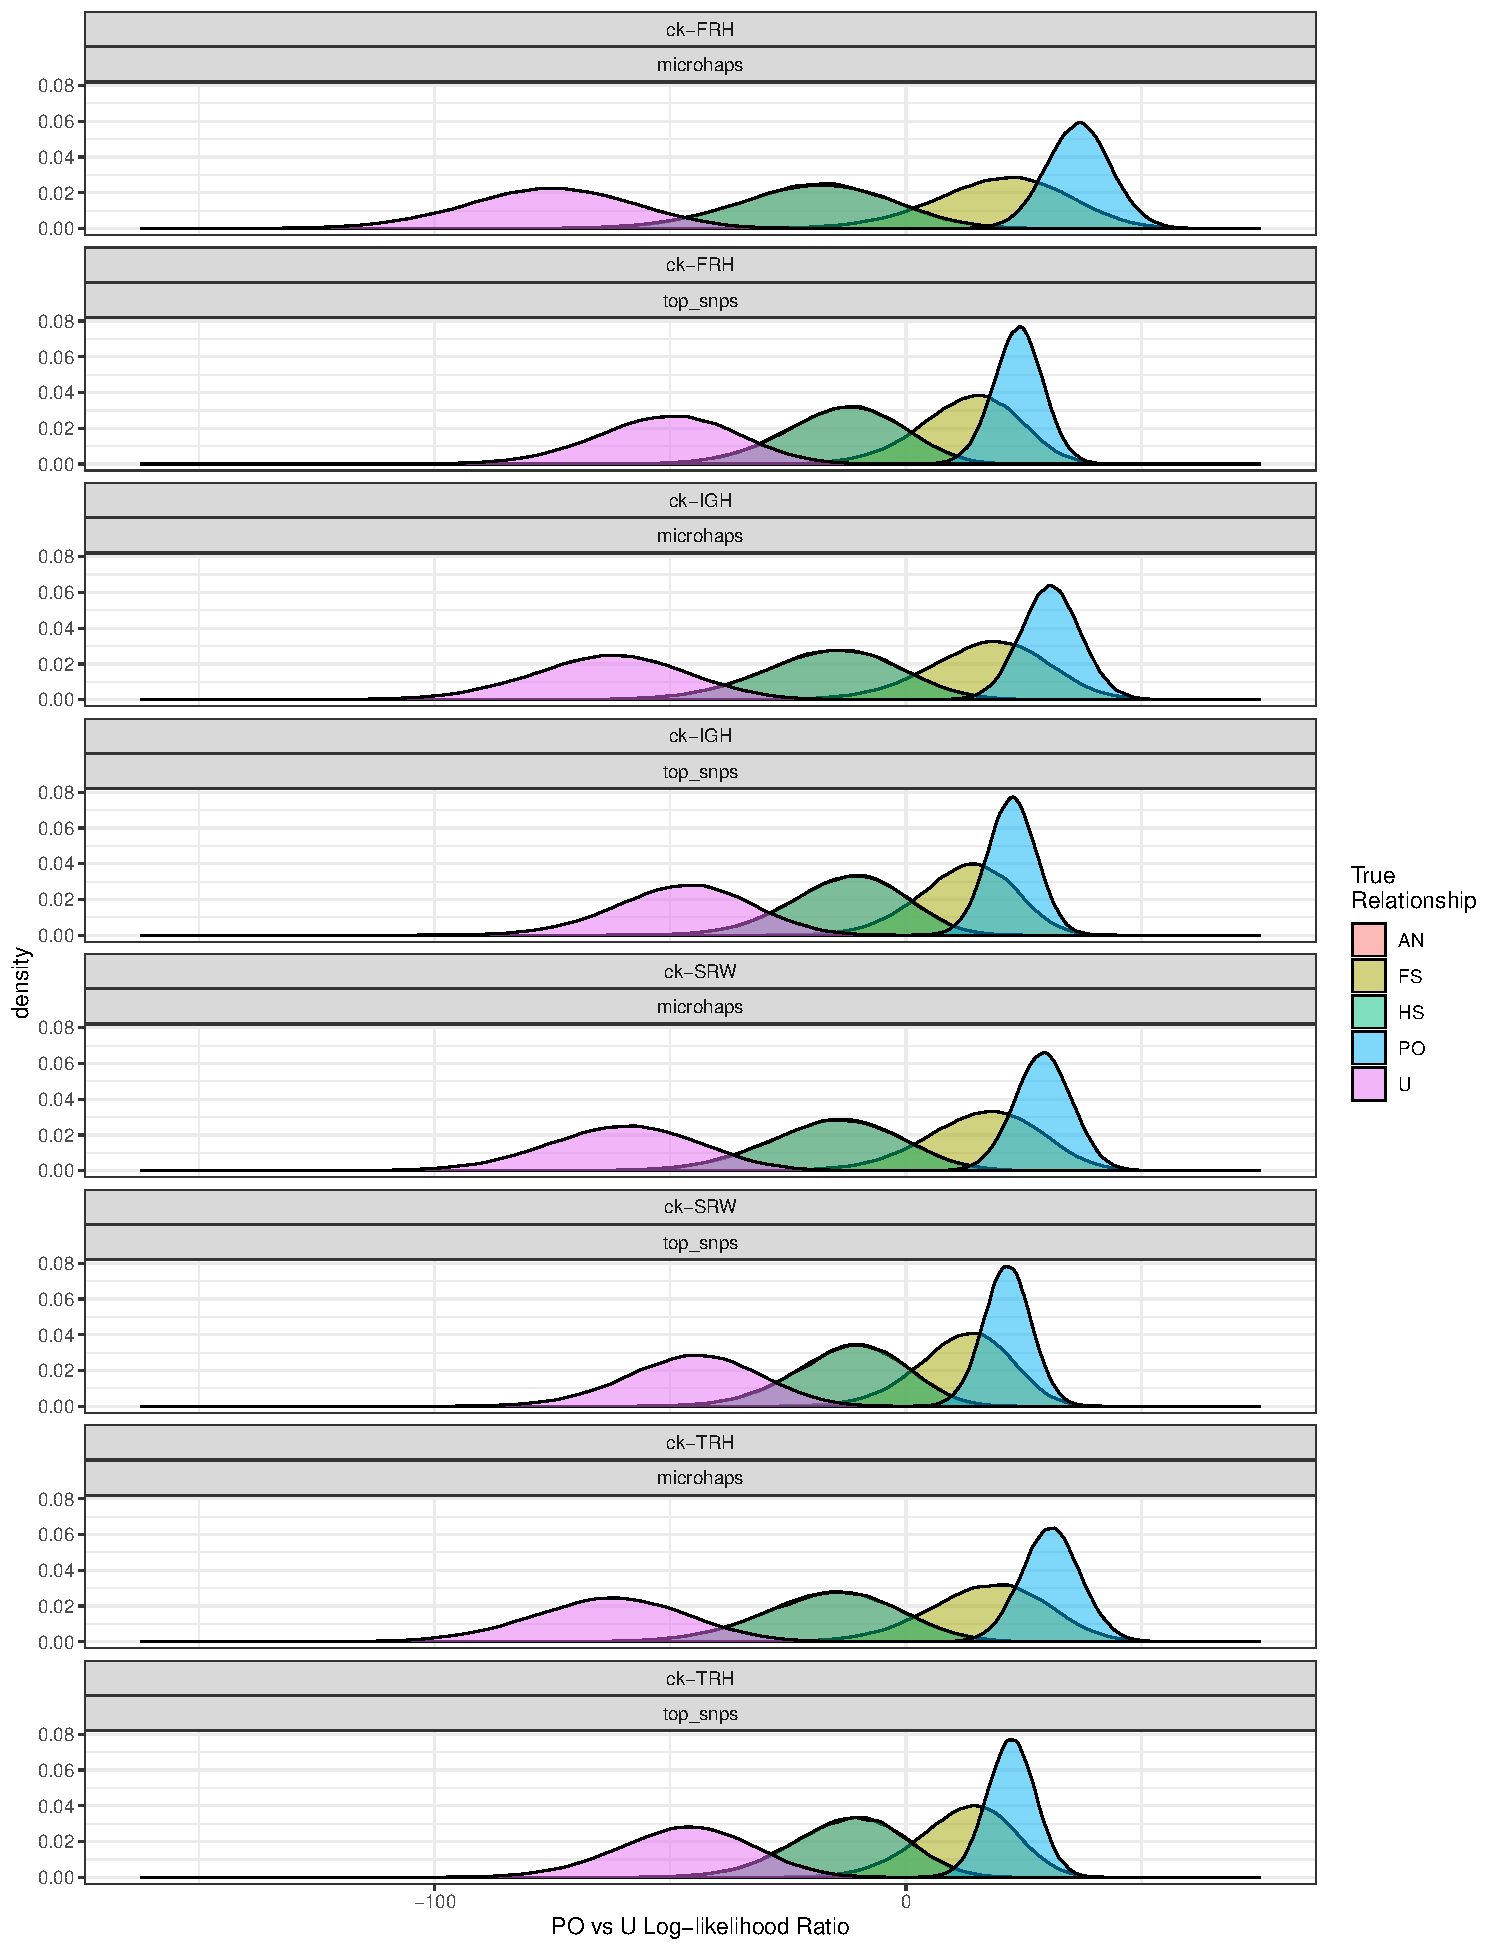
\includegraphics[width=0.9\textwidth]{images/cmkr-comp-figure-crop.pdf}
\end{center}
\caption[Comparison of microhaplotypes vs.~best SNP in each amplicon]{\footnotesize 
A comparison of the distribution of log-likelihood ratios when using all the alleles at each
amplicon typed as microhaplotypes ("microhaps" in the panel headers) versus using just a single (the most informative) SNP from each
amplicon ("top\_snps" in the panel headers).  Results shown for four hatchery collections in California 
(ck-FRH: Feather River Hatchery [spring and fall]; ck-IGH: Iron Gate Hatchery; ck-SRW: Sacramento Winter Run;
ck-TRH: Trinity River Hatchery [spring and fall]).  The density plots show
the distribution of log-likelihood ratios for Parent-Offspring vs Unrelated for four different relationships:
PO = parent offspring; FS = full-sibling; HS = Half sibling; AN = avuncular (i.e., aunt-niece, etc.)
The distributions for AN and HS overlap completely.  Note that the overlap between FS and PO occurs
for the PO vs U likelihood ratio, but is nearly eliminated with the PO vs FS likelihood ratio, allowing these
two relationships to be resolved accurately.}
\label{fig:ckmr-comp}
\end{figure}
%%%%%%%%%%%%%%%%%%%%




%%%%%%%%%%%%%%%%%%%
\begin{figure}
\includegraphics[width=\textwidth]{images/winter-v-non-winter-mh-plot_nind_ge10.pdf}
\caption[
	Absolute difference in allele frequency between winter run and non-winter run fish
]{
	\footnotesize Absolute difference in allele frequency between winter run and non-winter run fish of the CCV.
	The plot shows only those SNPs with at least a frequency difference of 0.5 between the two groups. Each point
	is a SNP. The  $x$ axis shows position in the Otsh\_v1.0 genome
	with color alternating by chromosome as indicated by RefSeq names on plot.
}
\label{fig:wrap-absdiff}
\end{figure}



%%%%%%%%%%%%%%%%%%%
\begin{figure}
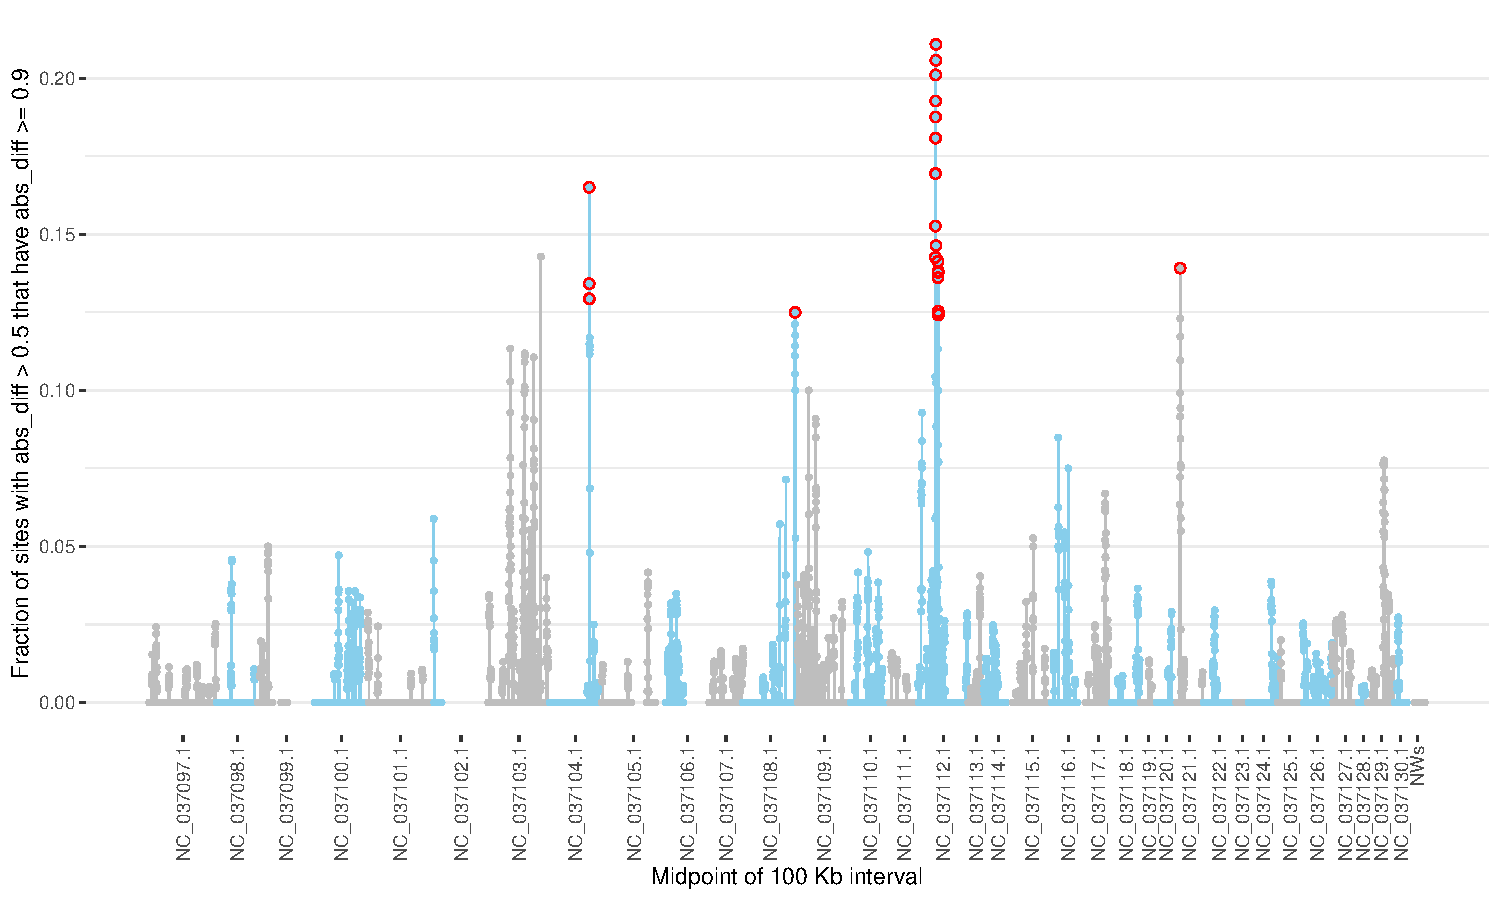
\includegraphics[width=\textwidth]{images/wrap-slide-window.pdf}
\caption[
	Sliding windows of absolute allele frequency difference between winter run and others
]{
	\footnotesize Values within 100 kb sliding windows of the fraction of sites with $|d|$ (absolute difference in
	allele frequency between winter run and non-winter run fish of the CCV) greater than 0.5 that also have
	$|d|>0.9$. The  $x$ axis shows position in the Otsh\_v1.0 genome
	with color alternating by chromosome as indicated by RefSeq names on plot. Red circles denote sliding
	windows chosen for further investigation for candidate markers.
}
\label{fig:wrap-slide-window}
\end{figure}





%%%%%%%%%%%%%%%%%%%
\begin{figure}
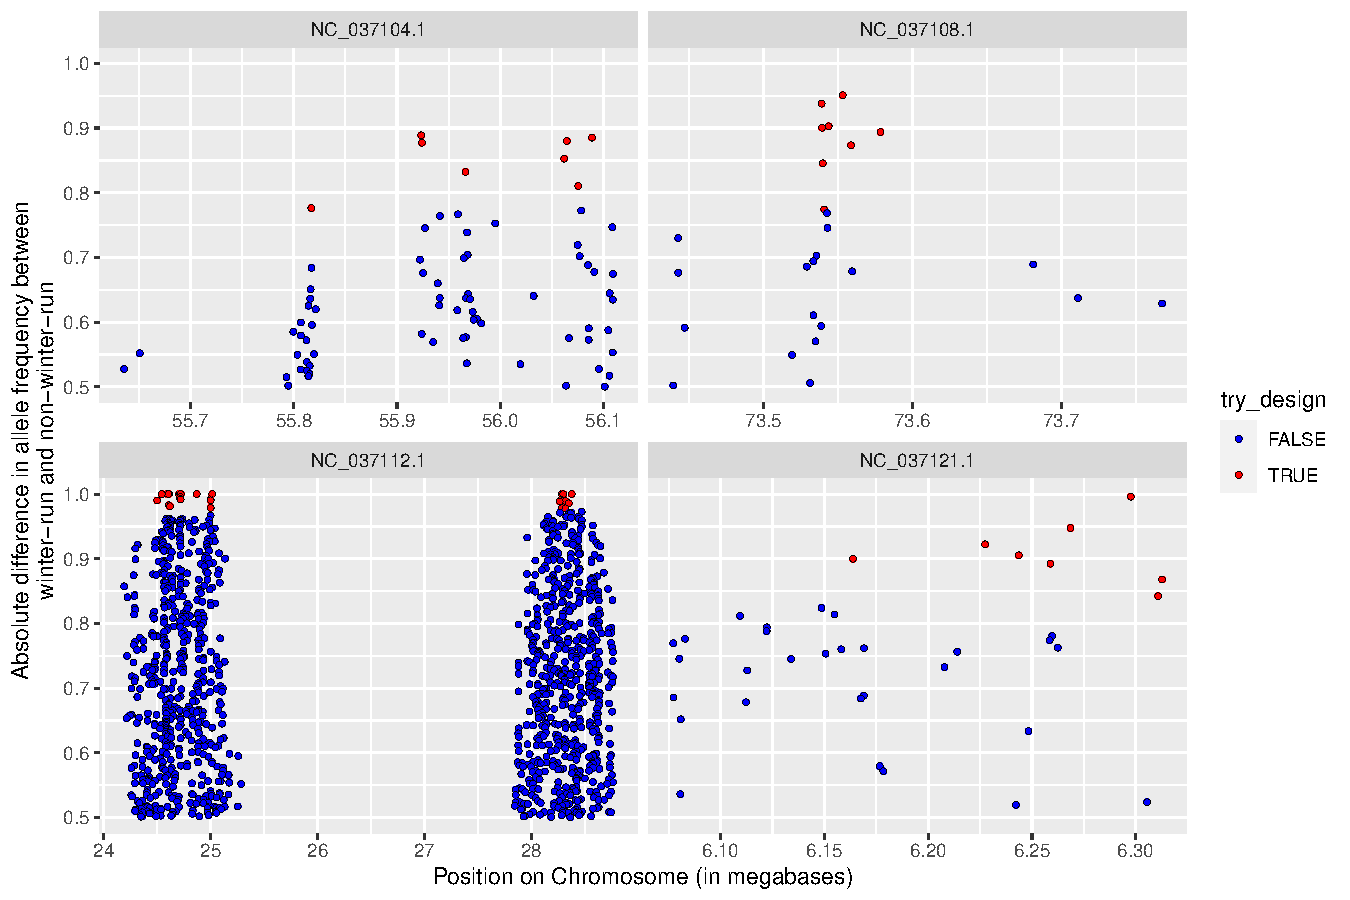
\includegraphics[width=\textwidth]{images/wrap-candi.pdf}
\caption[
	61 candidates for primer design for winter-run-associated polymorphisms
]{
	\footnotesize Genomic positions and values of $|d|$ (absolute difference in
	allele frequency between winter run and non-winter run fish of the CCV)
	for the 61 candidate SNPs (in red) to design for winter-run-associated polymorphisms
	(WRAPs).  Other sites are shown in black.  The $x$-axis shows position on
	each chromsome in the Otsh\_v1.0 assembly.  The chromsome name is indicated in the facet headers by
	RefSeq name
}
\label{fig:wrap-candi}
\end{figure}


\clearpage

{\small
%!TEX root = supplement.tex



%%%%%%%%%%%%%%
\begin{table}
\caption[Allele frequencies of winter-run-associated polymorphisms]{Allele frequencies across reporting units of the three winter-run associated
markers. Genome coordinates of SNPs are from Otsh\_v2.0. Alleles are listed according to the SNP nucleotide
at the variable SNPs within the amplicon.}
\label{tab:wrap-freqs}
{\footnotesize
\begin{tabular*}{\columnwidth}{@{\extracolsep{\fill}} lrrrrrrrr}
\hline\hline
Locus&Allele&CV-Winter&CV-Spring&CV-Fall&CV-Late-Fall&Cent-Cal-Coast&Klamath-Trinity&SO-NCal-Coast \\ \hline
Chr08:27450181&C&0.838&0.257&0.088&0.039&0.015&0.022&0.016\tabularnewline
Chr08:27450181&A&0.162&0.743&0.912&0.961&0.985&0.978&0.984\tabularnewline
Chr12:70794116&GAA&0.815&0.032&0.033&0.017&0.000&0.000&0.000\tabularnewline
Chr12:70794116&GAT&0.149&0.860&0.817&0.734&0.700&0.720&0.686\tabularnewline
Chr12:70794116&AAT&0.032&0.087&0.142&0.234&0.022&0.026&0.024\tabularnewline
Chr12:70794116&GTT&0.005&0.021&0.008&0.015&0.278&0.254&0.291\tabularnewline
Chr16:36409831&CCG&0.797&0.026&0.007&0.003&0.000&0.009&0.192\tabularnewline
Chr16:36409831&TCG&0.162&0.263&0.336&0.437&0.195&0.430&0.371\tabularnewline
Chr16:36409831&TCA&0.036&0.616&0.610&0.507&0.485&0.547&0.415\tabularnewline
Chr16:36409831&TGG&0.005&0.095&0.048&0.053&0.320&0.015&0.022\tabularnewline

\end{tabular*}
}
\vspace*{-2.3ex}\hrule\vspace*{0.3ex}\hrule
\end{table}
%%%%%%%%%%%%%%%

\clearpage



\bibliographystyle{men}
{\footnotesize
\bibliography{citation}}


%\appendix
%
%{
%\small
%\input{appendix}
%}

\end{document}


